\documentclass[a4paper,11pt,final]{article}
% Pour une impression recto verso, utilisez plutôt ce documentclass :
%\documentclass[a4paper,11pt,twoside,final]{article}

\usepackage[english,francais]{babel}
\usepackage[utf8]{inputenc}
\usepackage[T1]{fontenc}
\usepackage[pdftex]{graphicx}
\usepackage{setspace}
\usepackage{hyperref}
\usepackage[french]{varioref}
\usepackage[left=3cm,right=3cm,bottom=2cm,top=2cm]{geometry}
\usepackage{amssymb}
\usepackage{amsthm}


\usepackage[active,tightpage]{preview}

\usepackage{stmaryrd}

\usepackage{tikz}
\usepackage{pgf}
\usetikzlibrary{matrix}
\usetikzlibrary{calc}
\usetikzlibrary{fit}
\usetikzlibrary{arrows,automata}
\usetikzlibrary{automata,positioning}
\usetikzlibrary{shapes.multipart}

\tikzstyle{every loop}=[->,shorten >=1pt,looseness=8]
\tikzstyle{loop above}=[in=135,out=45,loop]


\newcommand{\reporttitle}{Validation de stabilité d'un système hybride}     % Titre
\newcommand{\reportauthor}{M.~Romain \textsc{Pichard}} % Auteur
\newcommand{\reportsubject}{Stage de fin d'étude} % Sujet
\newcommand{\HRule}{\rule{\linewidth}{0.5mm}}
\setlength{\parskip}{1ex} % Espace entre les paragraphes

\hypersetup{
    pdftitle={\reporttitle},%
    pdfauthor={\reportauthor},%
    pdfsubject={\reportsubject},%
    pdfkeywords={rapport} {vos} {mots} {clés}
}

\theoremstyle{plain}
\newtheorem{theo}{Théorème}

\theoremstyle{definition}
\newtheorem{definition}{Définition}

\theoremstyle{remark}
\newtheorem{rem}{Remarque}

\begin{document}
  % Inspiré de http://en.wikibooks.org/wiki/LaTeX/Title_Creation

\begin{titlepage}

\begin{center}

\begin{minipage}[t]{0.48\textwidth}
  \begin{flushleft}
    
\includegraphics [width=30mm]{images/logo_univ_tlse.png} \\[0.5cm]
  \end{flushleft}
\end{minipage}
\begin{minipage}[t]{0.48\textwidth}
  \begin{flushright}
    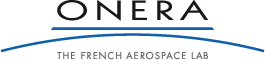
\includegraphics [width=50mm]{images/onera.png} 
  \end{flushright}
\end{minipage} \\[1.5cm]

\textsc{\Large \reportsubject}\\[0.5cm]
\HRule \\[0.4cm]
{\huge \bfseries \reporttitle}\\[0.4cm]
\HRule \\[1.5cm]

\begin{minipage}[t]{0.32\textwidth}
  \begin{flushleft} \large
    \emph{Auteur :}\\
    \reportauthor
  \end{flushleft}
\end{minipage}
\begin{minipage}[t]{0.6\textwidth}
  \begin{flushright} \large
    \emph{Responsables :} \\
    M.~Xavier \textsc{Pucel} \\
    M.~Thomas \textsc{Loquen}
  \end{flushright}
\end{minipage}

\vfill

{\large \today}

\end{center}

\end{titlepage}

  \cleardoublepage % Dans le cas du recto verso, ajoute une page blanche si besoin
  \tableofcontents % Table des matières
  \sloppy          % Justification moins stricte : des mots ne dépasseront pas des paragraphes
  
\cleardoublepage

%\section{Remerciements}

\section{La planification}
\subsection*{Introduction}
Le but de cette note est d'établir un état de l'art sur notre problème de planification de mission pour un drone. Nous cherchons à développer une méthode permettant la génération d'un plan faisable par le drone, c'est à dire que l'engin ne doit pas se retrouver dans une situation d'instabilité.

\subsection{Les différentes méthodes de planification}

\subsection{La planification appliquée aux mission de drone}
\cite{CHA05} présente une architecture très intéressante pour le problème de planification de mission pour un drone : 
\begin{itemize}
	\item niveau 3 : gestion de la mission et de son environnement, ce niveau permet de prendre en compte une modification de l'environnement de mission du drone, et donc de demander un nouveau plan (niveau 2)
	\item niveau 2 : Gestion du plan, ce niveau permet le calcul effectif d'un plan (demandé par le niveau 3, ou le niveau 1 si un segment du plan n'est pas conforme)
	\item niveau 1 : Gestion de la trajectoire, ce niveau permet le calcul d'une trajectoire pour le segment de plan donné par le niveau 2, il doit ressortir l'ensemble des points que doit suivre le drone pour réaliser ce segment du plan, si le niveau 0 considère que le prochain point n'est pas atteignable, le niveau 1 doit calculer une nouvelle trajectoire pour ce même segment
	\item 0 : guidage, ce niveau permet le guidage du drone, il doit informer le niveau 1 si le prochain point est atteignable ou pas, si il l'est, il demande à la couche de commande d'effectuer les actions nécessaires pour aller à ce point (modification de l'angle d'incidence, augmentation de la poussée etc...
\end{itemize}
Dans ce travail, les niveaux 3 et 2 ont était traité, les niveaux inférieurs ont était considéré comme connu. Le niveau 1 peut être vu comme du motion planning (un drone est vu comme un robot non-holonome), le niveau 0 lui peut être vu comme la boucle de commande du drone (modélisation continu, contraintes LMIs pour la stabilité), mais cette commande doit intégrer des aspects discret (mission) et continu (mécanique du vol, stabilité), nous pouvons donc émettre l'hypothèse qu'un modèle hybride serait utile.

Dans le monde de la robotique il existe une sous branche du motion planning : Kinodynamic planning, c'est à dire que l'on va prendre en compte (dès la phase de planification) la dynamique du robot (contrainte non-holonome, stabilité ...)
Alors qu'avec l'architecture proposée dans \cite{cha05}, le niveau 2 donne un plan non contraint par la dynamique, le niveau 1 donne une trajectoire elle aussi non contrainte par la dynamique, et c'est seulement le niveau 0 qui est capable de faire remonter des informations sur l'aspect réalisable du mouvement ou pas.

%\subsection{Thèse DICHEVA 2012}
\cite{DIC12} Ce travail de thèse porte une attention soutenue à la planification de mission pour le drone Eole. Il permet d'avoir un état de l'art récent sur les aspects de planification pour drone, ainsi que pour les architectures de mission.

L'architecture proposée est globalement la même que celle de CHANTERY vue ci-dessus, mais dans ce travail tout les niveaux ont était traité (Cf. page 180) : 
\begin{itemize}
	\item niveau 2 : Planification de mission : Un algorithme A* en 3D est proposé (avec une extension "4D" pour intégrer le temps). Cette planification peut-être apparenté à la KinoDynamic planning car l'auteur prends en compte dans ce niveau du rayon minimal de virage ainsi que la pente maximale.
	\item niveau 1 : Génération de trajectoire : Cette partie est solutionnée par l'utilisation de polynômes cartésiens d'ordre 3
	\item niveau 0 : Suivi de trajectoire : Cette étape est réalisée en utilisant une commande par mode glissant.
	\item niveau 0 bis : Modélisation de l'aéronef
\end{itemize} 

Le chapitre 5 de ce travail détaille le niveau 0 (suivi de trajectoire), car il est lui même décomposé de 4 éléments distincts.

Dans ce travail l'algorithme de planification est très intéressant car il permet la prise en compte d'un plan 3D, la modélisation de Eole est assez détaillée, de plus la prise en compte d'un modèle météo a été effectuée.

Mais ce travail, même s'il résout le problème de planification pour un drone, suppose que les restrictions faites au niveau 2 (KinoDynamic) sont suffisante pour assurer la stabilité du drone sur l'ensemble du plan.



%%\phantomsection\addcontentsline{toc}{section}{Références}
\begin{thebibliography}{ABC}	
    \bibitem{kur02} Monika KUROVSKY. \emph{Etude des systèmes dynamiques hybrides par représentation d'état discrète et automate hybride.}. Institut National Polytechnique Grenoble - INPG, 2002.
    \bibitem{cha05} Elodie CHANTERY. \emph{Planification de mission pour un véhicule aérien autonome}. École nationale supérieure de l'aéronautique et de l'espace, 2005.
    \bibitem{art06} Christian ARTIGUES, Dominique FEILLET. \emph{Une méthode exacte pour le problème d'ordonnancement d'atelier avec temps de préparation}. Écoles des Mines d'Alès, 2006.
    \bibitem{her07} Florent HERNANDEZ. \emph{Model-chechking et ordonnancement : Application à la décision de protection phytosanitaire de la vigne}. CEMAGREF, 2007.
    \bibitem{yalmip} Johan LÖFBERG. \emph{A toolbox for modeling and optimization in MATLAB}. Automatic Control Laboratory, 2004.
    \bibitem{goe09} Goebel, R. ; Sanfelice, R.G. et Teel, A. \emph{Hybrid dynamical systems : Robust stability and control for systems that combine continuous-time and discrete-time dynamics}. IEEE Control Systems, 2009.
    \bibitem{boy94} S. BOYD, L. El GHAOUI, E. FERON, V. BALAKRISHNAN. \emph{Linear matrix inequalities in system and control theory}. SIAM, 1994.
	\bibitem{arz08} Denis ARZELIER. \emph{Course on LMI optimization with applications in control : part II.1 and II.2}. LAAS, 2008.
	\bibitem{dic12} Svetlana DICHEVA. \emph{Planification de mission pour un système de lancement aéroporté autonome}. Université d’Evry-Val d’Essonne, 2012.
\end{thebibliography}



%\end{document}


\section{Notre problème}
Les deux travaux présentés précédemment présentent deux points de vue différent pour le problème de planification de drone, DICHEVA propose un aspect KinoDynamic planning et CHANTERY propose une communication verticale descendante et ascendante à tous les étages (Le dernier étage prévient de précédent si ses entrées ne correspondent pas à son domaine de définition).
DICHEVA assure la faisabilité de la mission mais n'assure pas la stabilité en tout point, CHANTERY propose une architecture permettant l'étude de la stabilité mais ne l'a pas traitée.

Une idée serait de fusionner plusieurs résultats de chacun de ces travaux et d'y apporter un aspect de stabilité. Une solution pourrait-être d'utiliser la planification basé sur le A* 3D de DICHEVA dans une architecture plus proche de celle de CHANTERY, en effet celle-ci nous permettrai de modifier le niveau 0 afin qu'il puisse faire remonter les problèmes de stabilité aux étages supérieurs.
Pour ce faire une proposition est de modéliser la commande du drone par un modèle hybride (automate hybride), celui-ci aurait pour but de vérifier que le prochain point de la trajectoire (niveau 1) est atteignable stablement. Le modèle hybride permet de prendre en compte les aspects continu du drone ainsi que les aspects discrets induit par la planification.
En d'autre terme, l'automate hybride pourrait être un graphe de changement de mode (régime de vol). Un exemple est donné sur la figure \ref{exempleGraphe}.
\begin{center}
	\begin{figure}[h]
	
		\[	
		\begin{tikzpicture}[->,>=stealth',shorten >=1pt,auto,node distance=2.8cm,
		semithick,every text node part/.style={align=center}]
		\tikzstyle{every state}=[fill=white,draw=black,text=black]
		
		
		\node   (A)   at (2,1.5)  {};
		\node[state]    (B)  at (3,0)     {mode 1 \\ maintien \\ $\alpha = 0$};
		\draw[<-] (B) to[bend right] (A)  ;
		
		\node[state]    (C)   at (0,-4)     {mode 2 \\ aquisition \\ $|\alpha| \leq 20$};
		\node[state]    (D)   at (6,-4)     {mode 3 \\ piqué \\ $-45 \leq \alpha \leq -20$};
		
		\path 
		(B) edge [bend left=10] node {$Z_{cons} = z$}   (C)
		
		(C) edge [bend left=10] node {$Z_{reel} == z$}   (B)		
		(C) edge [bend left=10] node {$\alpha \leq -20$}   (D)	

		(D) edge [bend left=10] node {$\alpha \geq -20$}  (C)	
		(D) edge [bend right=10] node {$Z_{reel} == z$}  (B);		

		
		\end{tikzpicture} 
		\]
	\caption{Exemple d'automate hybride}
	\label{exempleGraphe}
	\end{figure}
\end{center}

Une fois le modèle du drone établit, nous devons générer un plan en fonction de la mission voulu qui soit à la fois réalisable et stable. La figure \ref{scenario} représente un scénario, sur celui-ci est présent des obstacle à éviter.

\begin{figure}
	\centering
	
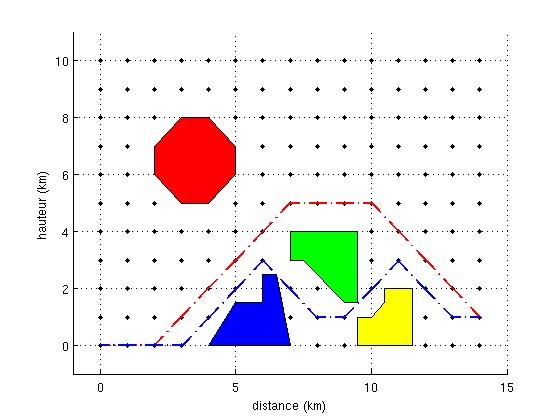
\includegraphics[scale=0.6]{images/scenario.jpg}
\caption{Scenario d'une mission (rouge : dijkstra, bleu : bellman)}
\label{scenario}
\end{figure}

A partir de ce plan (point de passage), il nous faut établir l'enchainement de mode (ainsi que la durée de chacun) permettant la suivi de ce plan.
Une fois cet enchainement effectué, nous devons étudier la stabilité du plan, c'est à dire vérifier que à tout instant, chaque mode est stable, et chaque changement de mode est possible.

Si l'étude de stabilité est effectué sur le plan de la figure \ref{scenario}, le trajet bleu doit poser problème car l'angle d'incidence dépasse la limitation. A partir de ce moment là, nous devons générer des conditions, de façon automatique, permettant le calcul d'un nouveau plan. Cette démarche doit être effectuée tant que le plan n'est pas entièrement stable et que l'objectif n'est pas atteint.


\section{Éléments de stabilité}
\subsection*{Introduction}
Le but de cette partie est d'apporter des éléments généraux mais nécessaires à la compréhension et à la réussite de mon travail de stage. Dans un premier temps quelques rappels seront effectués sur la modélisation d'un système linéaire par espace d'état, puis sur les notions d'équilibre et de stabilité de ces systèmes. Ensuite nous introduirons les notions de stabilité au sens de Lyapunov. Enfin nous ferons un point sur les inéquations linéaires matricielles (LMI en anglais), qui nous seront utiles pour Lyapunov. %Nous finirons par les outils d'analyse à notre disposition.

\subsection{Systèmes Linéaires}

\begin{definition} Modèle d'état\\
\label{defmodeleEtat}
Soit un système vérifiant les hypothèses de linéarité, sa représentation d'état est donnée par : 
\[\dot{X}(t) = A(t).X(t) + B(t).U(t)\]
\[Y(t) = C(t).X(t) + D(t).U(t)\]
$X(t) \in \mathbb{R}^{n}$ est le vecteur d'état;\\
$Y(t) \in \mathbb{R}^{r}$ est le vecteur de sortie;\\
$U(t) \in \mathbb{R}^{m}$ est le vecteur des entrées;\\
$A(t) \in \mathbb{R}^{n\times n}$ est la matrice dynamique;\\
$B(t) \in \mathbb{R}^{n\times m}$ est la matrice de commande;\\
$C(t) \in \mathbb{R}^{r\times n}$ est la matrice de mesure ou de sortie;\\
$D(t) \in \mathbb{R}^{r\times m}$ est la matrice de transmission directe,
\end{definition}
Dans le cas général, un tel système est appelé système Linéaire à Temps Variant (LTV). Dans les cas particuliers où A, B, C et D sont constantes, le système est dit Linéaire à Temps Invariant (LTI).
Dans la suite nous considérerons les systèmes LTI.

\subsubsection{Notions de stabilité}
Parler de la stabilité d'un système est un abus de langage, en réalité nous devons parler de la stabilité d'un point d'équilibre, de fonctionnement ou d'une trajectoire de ce système.

\begin{definition} État d'équilibre\\
	\label{defEtatEq}
Un point $X_e$ de la trajectoire d'état est un état d'équilibre (point d'équilibre) si $X(t_0) = X_e \Leftrightarrow X(t) = X_e, \forall t \geq t_0$ en l'absence de commande et de perturbations.\\
Pour une représentation d'état comme vu précédemment, les points d'équilibre sont les solutions de l'équation : 
\[\dot{X}(t) = 0_{n,1} \Leftrightarrow A.X(t) = 0_{n,1}\]
\end{definition}


\begin{theo}
	\label{theoAinversible}
Un système continu LTI d'équations $\dot{X}(t) = A.X(t)$ peut avoir\\
- Un point d'équilibre unique X = 0 si A est inversible\\
- Une infinité de points d'équilibre si A n'est pas inversible	
\end{theo}

La stabilité permet de caractériser les points d'équilibre du système, c'est à dire que, si à un instant $t_0$, l'état d'équilibre est perturbé, l'état reviendra-t-il à cet état d'équilibre (stabilité) ou divergera-t-il (instabilité) ? Les différents types de stabilité sont présentés ci-après.

\begin{definition} Stabilité interne\\
	\label{defInterne}
L'état d'équilibre $X_e$ est dit \textbf{stable} si
\[ \forall \epsilon > 0, \exists\alpha > 0 \emph{ tel que si } ||X(0) - X_e|| \leq \alpha \emph{ alors } ||X(t) - X_e|| \leq \epsilon \]	
Dans le cas contraire, $X_e$ est dit \textbf{instable}.
\end{definition}

\begin{definition} Stabilité asymptotique\\
	\label{defAsymp}
L'état d'équilibre $X_e$ est dit \textbf{asymptotiquement stable} si
\[ \exists\alpha > 0 \emph{ tel que si } ||X(0) - X_e|| \leq \alpha \emph{ alors } \lim\limits_{t \rightarrow +\infty} X(t) = X_e \]
\end{definition}

\begin{definition} Stabilité exponentielle\\
	\label{defExpo}
L'état d'équilibre $X_e$ est dit \textbf{exponentiellement stable} s'il existe $\alpha > 0$ et $\lambda > 0$ tels que 
\[ \forall t > 0, \exists B_r(X_e,r), \forall X_0 \in B_r, ||X(t) - X_e|| \leq \alpha||X(0) - X_e||e^{-\lambda t} \]
où $B_r$ est une boule fermée de $\mathbb{R}^n$
\end{definition}

\begin{rem}
	\label{remImplique}
Il est possible de montrer que :
\begin{center}
stabilité exponentielle $\Rightarrow$ stabilité asymptotique $\Rightarrow$ stabilité interne
\end{center}
\end{rem}

Pour finir sur les notions de stabilité d'un système LTI, nous allons regarder la caractérisation de la stabilité. Soit le point d'équilibre $X_e$ du système décrit par un modèle d'état comme présenté à la définition \ref{defmodeleEtat}, alors la caractérisation de la stabilité s'étudie à partir de la matrice A. A possède r valeurs propres distinctes $\lambda_1,\ldots,\lambda_r$. Et nous avons le théorème suivant : 
\begin{theo} Conditions sur les valeurs propres\\
$Re(\lambda_i) > 0$ si il existe $i \in 1,\ldots,r$, alors $X_e$ est \textbf{instable}\\
$Re(\lambda_i) \leq 0$ pour tout $i \in 1,\ldots,r$, alors :\\
\vspace{-1cm}
\begin{tabbing}
	\hspace{1cm}\=\kill
	\> $Re(\lambda_i) < 0$ pour tout $i \in 1,\ldots,r$, alors $X_e$ est \textbf{asymptotiquement stable};\\ 
	\> $Re(\lambda_i) = 0$ et A diagonalisable, alors $X_e$ est \textbf{stable};\\ 
	\> $Re(\lambda_i) = 0$ et A non-diagonalisable, alors $X_e$ est \textbf{instable}.
\end{tabbing} 
\end{theo}

\subsubsection{Méthode directe de Lyapunov pour l'étude de stabilité}
Considérons la stabilité du point d'équilibre 0 pour les systèmes étudiés, en effet d'un point de vue physique, la méthode de Lyapunov s'apparente à regarder l'évolution de la fonction d'énergie. Donc étudier le point d'équilibre 0 est équivalent à étudier à quel moment le système n'aura plus d'énergie. 

Pour tout point d'équilibre $x_e \neq 0$, on pose le changement de variable \^{x}(t) = x(t)-$x_e$ et l'étude de la stabilité est identique à celle pour $x_e = 0$.
\begin{definition} Fonction candidate de Lyapunov\\
	\label{defFctLyap}
Soit $V : \mathbb{R}^n \rightarrow \mathbb{R}_+$ une fonction telle que : 
\begin{itemize}
\item[i)] V est continûment différentiable en tous ces arguments
\item[ii)] V est définie positive
\item[iii)] Il existe a et b deux fonctions de $\mathbb{R}_+$ dans $\mathbb{R}_+$, continues, monotones, non décroissantes, telles que
\[a(0) = b(0) = 0\]
\[\forall x \in \mathbb{R}^n a(||x||) \leq V(x) \leq b(||x||)\]
alors V est une fonction candidate de Lyapunov.
\end{itemize}
\end{definition}

\begin{rem}
La définition implique que la fonction V définit des équipotentielles imbriquées. C'est à dire que les courbes V(x) = cste, appelées \textbf{équipotentielles de Lyapunov}, définissent des domaines connexes autour de l'origine.
\end{rem}

\begin{theo} Stabilité locale\\
Si il existe une fonction $V$ dont les dérivées partielles premières sont continues et telle que :
\begin{itemize}
\item[1-] V est une fonction candidate de Lyapunov (Cf. définition \ref{defFctLyap})
\item[2-] $\dot{V}$ est localement semi-définie négative dans un voisinage de l'origine $\Omega$.
\end{itemize}

Alors le point d'équilibre 0 est \textbf{stable} et un domaine de conditions initiales stables est délimité par n'importe quelle équipotentielle de Lyapunov contenue dans $\Omega$.\\
Si $\dot{V}$ est localement définie négative dans $\Omega$, alors la stabilité est dite \textbf{localement asymptotique} dans la partie de l'espace délimitée par n'importe quelle équipotentielle de Lyapunov contenue dans $\Omega$.
\end{theo}

\begin{theo} Stabilité globale asymptotique\\
	\label{theoStabLyap}
S'il existe une fonction V telle que
\begin{itemize}
\item[1-] V est une fonction candidate de Lyapunov
\item[2-] $\dot{V}$ est définie négative
\item[3-] La condition $||x|| \rightarrow +\infty$ implique $V(x) \rightarrow +\infty$
\end{itemize}
alors 0 est un point d'équilibre globalement asymptotiquement stable.
\end{theo}

Le problème de cette méthode de Lyapunov est de trouver une fonction de Lyapunov pour le système considéré, en effet dans le cas non-linéaire il n'existe pas de méthode systématique. Dans le cas des systèmes LTI, il existe forcément une fonction de Lyapunov, mais elle n'est pas évidente à trouver.

\subsubsection{Application aux systèmes linéaires}
Dans ce cas, la représentation du système est donc classique : $\dot{x} = Ax$. Le point d'équilibre candidat est nécessairement $x = 0$. En choisissant $V(x) = x^TPx$ avec $P$ symétrique et définie positive ($P = P^T > 0$), la condition de stabilité asymptotique (Cf. Théorème \ref{theoStabLyap}) s'écrit alors 
\begin{center}
	$   \left \{
	\begin{array}{c c l}
	V(x) = x^TPx & > & 0, \forall x \\
	\dot{V}(x) = x^T(A^TP + PA)x & < & 0, \forall x
	\end{array}
	\right. $
\end{center}

\begin{theo}
Le système $\dot{x} = Ax$ est stable si et seulement si il existe une matrice définie positive P vérifiant le système LMI suivant : 
\begin{center}
$   \left \{
\begin{array}{r c l}
P & > & 0 \\
A^TP + PA & < & 0
\end{array}
\right. $
\end{center}
\end{theo}

\begin{theo}
	Dans le cas d'un système discret du type $x_{k+1} = Ax_k$, le théorème de stabilité devient (Lemme de Schur) :
	\begin{center}
		$   \left \{
		\begin{array}{r c l}
		P & > & 0 \\
		A^TPA - P & < & 0
		\end{array}
		\right. $
	\end{center}
	\label{theo:lyapDiscret}
\end{theo}

Par la suite nous travaillerons avec des systèmes LTI discret soumis à une commande, d'après les travaux de \cite{zhai_analysis_2007}, les conditions LMI deviennent : 
\begin{theo}
	Dans le cas d'un système discret du type $   \left \{
	\begin{array}{l}
	x_{k+1} = Ax_k + Bu_k \\
	y_k = Cx_k + Du_k
	\end{array}
	\right. $ :
	\begin{center}		
		$   \left \{
		\begin{array}{c c l}
		P & > & 0 \\
		\begin{bmatrix}
		A^TPA-P+C^TC	& A^TPB + C^TD \\ 
		B^TPA + D^TC	& B^TPB - I + D^TD  
		\end{bmatrix} & < & 0
		\end{array}
		\right. $
	\end{center}
	\label{theo:lyapDiscretAvecEntree}
\end{theo}
\subsubsection{Résumé pour l'étude de la stabilité}
\begin{itemize}
\item[1-] Trouver les points d'équilibre du système en résolvant Ax = 0
\item[2-] Linéariser le système autour des points d'équilibre pour évaluer la stabilité/instabilité des points d'équilibre (cette étape est souvent appelée première méthode de Lyapunov). Au voisinage d'un point d'équilibre $x_e$ :
\[\dot{x} = f(x) = A(x-x_e) + o(x-x_e)\]
Si la matrice A est définie négative, le système est localement asymptotiquement stable autour de $x_e$, mais aucun domaine de conditions initiales stables ne peut-être déterminé à ce stade.
Si A est semi-définie négative, on ne peut pas conclure. Sinon le point d'équilibre est instable.
\item[3-] Choisir une fonction candidate de Lyapunov V et, en posant le changement de variable \^{x} = x - $x_e$, étudier les domaines de stabilité/instabilité à l'aide de la seconde méthode de Lyapunov.
\item[4-] Si les résultats ne sont pas concluants, choisir une autre fonction de Lyapunov et recommencer.
\end{itemize}

%\subsubsection{Utilisation de MatLab pour l'étude de la stabilité (Lyapunov + LMI)}
%Cf. LyapunovLin.m pour un exemple de vérification de la seconde méthode de Lyapunov. Et voir switch\_test2.m pour avoir un exemple de projection des ellipses dans les différents plans de l'espace.
%
%\subsection{Éléments divers}
%Cette section va nous permettre de présenter différents points qui pourront être intéressants par la suite
%
%\subsubsection{D-stable}
%Une Matrice carré réelle A est dite (Hurwitz) D-stable si pour toute matrice diagonale positive D, la matrice DA est (Hurwitz) stable (à valeur propre strictement négative).
%
%Une matrice A est dites Hurwitz diagonalement stable si il existe une matrice positive P diagonale tel que A'P+PA est définie négative.
%
%A est Schur diagonalement stable si il existe une matrice positive P diagonale tel que A'PA-P est définie négative.
%
%Hurwitz diagonale stabilité est une condition suffisante pour la D-stabilité, mais l'inverse n'est vrai que pour une certaine classe de matrice. (Cf. On discrete-time diagonal and D-stability)


%\end{document}


\chapter{Bibliographie}
\section{Systèmes hybrides}

Cette partie a pour but de présenter les systèmes dynamiques hybrides, leurs problématiques, les différentes classes de systèmes hybrides ainsi que les différents outils de modélisation.
Nous nous appuierons fortement sur le travail de thèse de \cite{Kur02}, et plus particulièrement les parties 1.1 à 1.3. Étant donné que l'étude détaillée est faite dans ce travail de thèse, je me contenterai de résumer ici les principales idées.

\subsection{Problématique}
Les systèmes automatisés actuels, de part leur complexité ne peuvent plus être représentés uniquement par leur comportement continu ou leur comportement discret, de nombreux systèmes réels sont à dynamique continue, mais supervisés ou contrôlés par une dynamique discrète. La modélisation de ces systèmes nécessitent une nouvelle approche et de nouveaux outils, c'est pourquoi ces dernières années de nombreux travaux vont dans ce sens et tentent de proposer des outils de modélisation et d'analyse.

\subsection{Classe de système hybride}
La nature hybride d'un système peut être inhérente aux phénomènes physiques qui le régissent, ou bien provoquée par une supervision de ce système. Il existe donc différentes classes de système hybride parmi lesquelles : 
\begin{itemize}
	\item \emph{Commutation autonome} : Caractérise un système qui va changer de façon discontinue lorsque l'état atteint certains seuils, c'est le cas des systèmes à hysteresis, la table de billard en est un exemple concret.
	\item \emph{Commutation contrôlée} : Traduit un phénomène où le système change de façon discontinue et instantanée en réponse à une entrée de commande, par exemple un système de thermostat. 
\end{itemize}

\subsection{Automate hybride}
La modélisation des systèmes dynamiques hybrides est un problème toujours en étude à ce jour \cite{goebel_hybrid_2012}. Le but est de réussir à trouver des outils permettant la représentation des dynamiques discrètes et continues dans une même syntaxe. L'automate hybride \cite{henzinger_theory_2000} est aujourd'hui un outil permettant de répondre à ces besoins. En effet, dans le domaine discret on représente très souvent les systèmes par un automate, en associant aux états des dynamiques continues, et en permettant aux transitions elles aussi des conditions continues, nous arrivons à modéliser un système dynamique hybride.

\begin{figure}[h]
	\centering	
	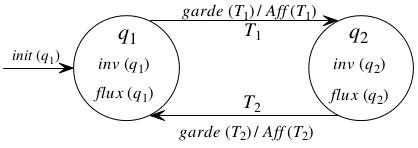
\includegraphics{images/automateHybride.jpeg}
	\caption{Automate hybride}
	\label{exempleAutomateHybride}
\end{figure}

L'\textit{état continu} du système est modélisé par un vecteur d'état continu $x(.)$ représentant un point dans un espace $X \subset \mathbb{R}^n$. Dans chaque sommet, la dynamique continue est modélisée par des conditions de flux telle que des équations différentielles ou des espaces d'états.

A chaque transition on associe un prédicat qui concerne l'état interne du système appelé \textit{garde}. Ce prédicat détermine les dates possibles pour le franchissement de la transition. Ainsi, une transition de l'automate hybride peut être franchie à l'instant $t$ si et seulement si sa garde est vérifiée par la valeur des variables d'état continues du système à l'instant considéré.

En général la garde d'une transition est exprimée par une région de l'espace d'état continu, qui peut se ramener à des intervalles.

L'ensemble des variables d'état continues mises à jour lors du franchissement d'une transition est décrit par une affectation. Les initialisations spécifiées par l'affectation correspondent à des fonctions, calculant la nouvelle valeur de l'état à partir de sa valeur avant le franchissement.

\begin{definition}{Un automate hybride d'ordre n, tel que présenté sur la figure \ref{exempleAutomateHybride} est défini par :}\\
\[\mathbb{A} = (Q, X, flux, inv, garde, Aff, init)\]
tel que :
\label{def:autom-hybride}
\begin{itemize}
\item Q = {$q_1, q_2, \ldots, q_m$} est un ensemble fini des sommets du graphe représentant les états discrets du système modélisé;
\item $X \subset \mathbb{R}^n$ est l'espace d'état continu. L'état continu du système est caractérisé à tout instant par le vecteur x = $[x_1, x_2, \ldots, x_n]^T$ dans l'espace Euclidien $\mathbb{R}^n$;
\item $flux(q_i)$ est la fonction qui affecte à chaque sommet une représentation pour l'évolution continue. Durant le séjour dans un sommet $q_i$ de l'automate hybride, l'évolution des variables continues est exprimée généralement sous la forme d'une équation d'état flux($q_i$) : $\dot{x} = \phi (q_i)(t,x,u)$, où $x \in X \subset \mathbb{R}^n$, $u \in U \subset \mathbb{R}^p$ et $\phi : X \times U \rightarrow X$;
\item L'invariant $inv(q_i)$ est une fonction qui associe à chaque sommet $q_i \in Q$ une contrainte sur les variables d'état continues x(.). Le système peut séjourner dans un sommet tant que l'invariant du sommet est satisfait;
\item $garde(T_i)$ est une fonction qui associe une condition de franchissement à chaque transition $T_i \in E$. Cette condition est en général une fonction logique entre des prédicats, portant sur les variables $x \in X$ et/ou ses dérivées $\dot{x} \in X$. Une transition $T_i \in E$ ne peut être franchie que si la condition $garde(T_i)$ est vraie;
\item L'affectation $Aff(T_i)$ est une fonction qui associe à chaque transition $T_i \in E$ une relation qui permet de mettre à jour la valeur des variables d'état après l'exécution de la transition $T_i$.
\item $init$ est une fonction qui affecte un état initial $x_0 \in X$ au sommet initial $q_{in} \in Q$. La condition initiale $init(q_{in})$ est un prédicat sur X.
\end{itemize}



\end{definition}


%\textbf{INSERER EXEMPLE SIMPLE : THERMOSTAT}

  %\cleardoublepage
  %%\phantomsection\addcontentsline{toc}{section}{Références}
\begin{thebibliography}{ABC}	
    \bibitem{kur02} Monika KUROVSKY. \emph{Etude des systèmes dynamiques hybrides par représentation d'état discrète et automate hybride.}. Institut National Polytechnique Grenoble - INPG, 2002.
    \bibitem{cha05} Elodie CHANTERY. \emph{Planification de mission pour un véhicule aérien autonome}. École nationale supérieure de l'aéronautique et de l'espace, 2005.
    \bibitem{art06} Christian ARTIGUES, Dominique FEILLET. \emph{Une méthode exacte pour le problème d'ordonnancement d'atelier avec temps de préparation}. Écoles des Mines d'Alès, 2006.
    \bibitem{her07} Florent HERNANDEZ. \emph{Model-chechking et ordonnancement : Application à la décision de protection phytosanitaire de la vigne}. CEMAGREF, 2007.
    \bibitem{yalmip} Johan LÖFBERG. \emph{A toolbox for modeling and optimization in MATLAB}. Automatic Control Laboratory, 2004.
    \bibitem{goe09} Goebel, R. ; Sanfelice, R.G. et Teel, A. \emph{Hybrid dynamical systems : Robust stability and control for systems that combine continuous-time and discrete-time dynamics}. IEEE Control Systems, 2009.
    \bibitem{boy94} S. BOYD, L. El GHAOUI, E. FERON, V. BALAKRISHNAN. \emph{Linear matrix inequalities in system and control theory}. SIAM, 1994.
	\bibitem{arz08} Denis ARZELIER. \emph{Course on LMI optimization with applications in control : part II.1 and II.2}. LAAS, 2008.
	\bibitem{dic12} Svetlana DICHEVA. \emph{Planification de mission pour un système de lancement aéroporté autonome}. Université d’Evry-Val d’Essonne, 2012.
\end{thebibliography}



\end{document}

